110. $y=\cfrac{x^2-8x+15}{|x-6|+|x-2|-2}=\begin{cases}
\cfrac{(x-5)(x-3)}{6-x+2-x-2}=\cfrac{5-x}{2},\ x<2,\\
\cfrac{(x-5)(x-3)}{6-x+x-2-2}=\cfrac{x^2-8x+15}{2},\ 2\leqslant x \leqslant 6,\\
\cfrac{(x-5)(x-3)}{x-6+x-2-2}=\cfrac{x-3}{2},\ 6<x.\end{cases}$
$$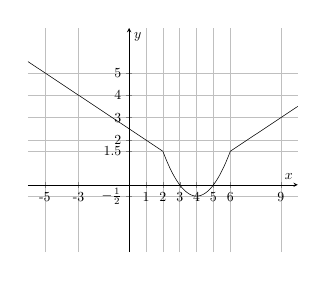
\begin{tikzpicture}[scale=0.5]
\begin{axis}[
    axis lines = middle,
    grid=major,
    legend pos={south west},
    xlabel = {$x$},
    ylabel = {$y$},
    ymin=-3,
    ymax=7,
    xtick={-5, -3 , 1, 2, 3, 5, 6, 9, 4},
    xticklabels={-5, -3 , 1, 2, 3, 5, 6, 9, 4},
    ytick={-0.5, 5, 4, 2, 1.5, 3},
    yticklabels={$-\frac{1}{2}$, 5, 4, 2, 1.5, 3}           ]
\addplot[domain=-6:2, samples=100, color=black] {(5-x)/2};
\addplot[domain=2:6, samples=100, color=black] {(x*x-8*x+15)/2};
\addplot[domain=6:10, samples=100, color=black] {(x-3)/2};
%\addplot[domain=-3.1:2.5, samples=100, color=red] {70*abs(1-2*abs(abs(x)-2))-10*x^2+10*x-70};
	%\addlegendentry{$\text{Рис. 1}$};
\end{axis}
\end{tikzpicture}$$
